\titre{Principe :} Avoir des pages de mémoire inscrites dans l'espace d'adressage de plusieurs processus.\\
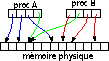
\includegraphics[width=200px]{fig19.pdf}

\titre{Avantage :} C'est le moyen le plus rapide d'échanger des données entre deux processus.\\

\titre{Inconvénient :} C'est aussi un très bon moyen pour créer des conditions de concurrence.\\

\titre{Comment ça marche ?} 
\begin{enumerate}
	\item Un processus crée un fichier virtuel (shm\_open)
	\item On redimensionne le fichier à la taille voulue (ftruncate)
	\item Projeter le fichier virtuel dans l'espace d'adressage du processus (mmap)
	\item Les processus qui veulent l'utiliser ouvrent le fichier (shm\_open) et le projettent dans leur espace d'adressage (mmap)
	\item Les processus utilisent cette mémoire partagée (attention aux conditions de concurrence)
	\item Lorsqu'un processus a terminé il ferme la projection (munmap) et le fichier (fclose)
	\item Lorsque tous les processus ont terminé, on détruit le fichier (shm\_unlink)
\end{enumerate}
